\documentclass{scrartcl}
\usepackage[utf8]{inputenc}
\usepackage[T1]{fontenc}
\usepackage[a4paper]{geometry}
\usepackage{graphicx}
\usepackage{hyperref}
\usepackage{float}
\usepackage{mathtools}
\usepackage{textcomp}
\usepackage{gensymb}
\usepackage[ngerman]{babel}
\usepackage{epstopdf}
\usepackage{titlesec}
\renewcommand{\arraystretch}{1.3}
\setcounter{secnumdepth}{5}
\setcounter{tocdepth}{5}
\makeatletter
\renewcommand\paragraph{\@startsection{paragraph}{4}{\z@}%
  {-3.25ex\@plus -1ex \@minus -.2ex}%
  {1.5ex \@plus .2ex}%
  {\normalfont\normalsize\bfseries}}
\newcommand*{\tline}{%
  \ifmeasuring@
  % first measuring run
  \else
  % second run
  % \typeout{\meaning\maxcolumn@widths}% debug info
  \ifodd\column@
  \expandafter\rlap
  \else
  \expandafter\llap
  \fi
     {%
       \vrule height-1ex depth \dimexpr1ex+.4pt\relax width
       \ifcase\numexpr\column@+1\expandafter\relax
       \maxcolumn@widths
       \fi
     }%
     \fi
}
\makeatother
\restylefloat{table}
\newcommand{\mytitle}{Übung 1}
\hypersetup{
  colorlinks=true,
  linkcolor=blue,
  pdftitle=\mytitle,
  pdfauthor={Fabian Nedoluha, Stefan Hermeter},
}
\begin{document}
\title{\mytitle:RegSim.c}
\subtitle{Bitverarbeitung}
\date{\today}
\author{Stefan Hermeter \texttt{\href{mailto:stefan.hermeter@gmx.at}{stefan.hermeter@gmx.at}}\\
  Klasse: 5ABETi\\
  Schuljahr: 2015/16, 28. November}
\pagenumbering{gobble}
\maketitle
\pagenumbering{roman}
\newpage
\tableofcontents
\listoffigures
\listoftables
\newpage
\pagenumbering{arabic}
\section{Aufgabenstellung}
Erstellen Sie ein Programm RegSim, welches ein Register simuliert bei dem die einzelnen Bits angesprochen werden können.\\
Das Programm sollte diese Aufgaben erfüllen:

%% Aufzählung der Anforderungen
\begin{itemize}
\item Register mit  \verb|\|x00 initialisieren
\item Bit 1 und Bit 5 auf 1 setzen
\item Einerkomplement bilden (reg = ~reg)
\item Bit 0 auf 1 setzen, alle anderen 0
\item alle Bits um 3 Stellen nach rechts (im Little - Endian - Sinne) verschieben
\item Register mit \verb|\|x00 XOR - verknüpfen
\item Register mit  \verb|\|\ xFF UND - verknüpfen
\end{itemize}
  
\subsection{Ausgabe}
Geben Sie nach jeder Aufgabenstellung den Wert des Registers als:

%% Aufzählung der Ausgabe
\begin{itemize}
\item[1)] Binär
\item[2)] Integerwert
\item[3)] Hexadecimal
\end {itemize}

\section{Programmablaufplan}
\section{Resourcen}

\subsection{Sourcecode-Files}
\begin{itemize}
\item RegSim.c
  \end{itemize}
\subsection{Verwendete Libraries}
\begin{itemize}
\item stdio.h
\end{itemize}
\section{Testergebnisse}
\subsection{Ausgabe}
\begin{figure}[H]
  \centering
  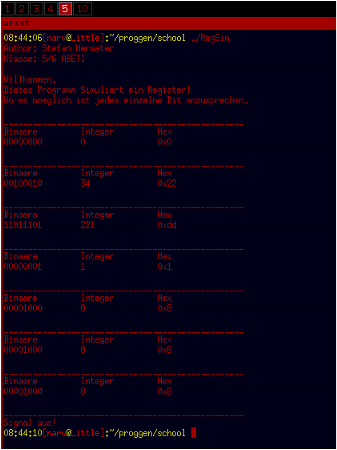
\includegraphics[width=\linewidth]{images/ausgabe1.png}
  \caption{Ausgabe}
  \label{fig:digraph}
\end{figure} 


\end{document}
